\section{Results}
\subsection{Live imaging of EB3 comets}
Because our experiment with the EB3 comets failed, we had to analyze the given prime example of the practical course.  
The analysis of the EB3-GFP movement was done with TrackMate \cite{Ershov_2021} \cite{Tinevez_2017} \\
It was assumed that the comet is $0.8\mu m$ long. The image was sampled at a rate of 2Hz. From this, TrackMate calculated the total travel length and the mean speed of each comet. (Fig. \ref{mt_live})

\begin{figure}[h!]
	\begin{center}
		\begin{minipage}{0,8\textwidth}
			
			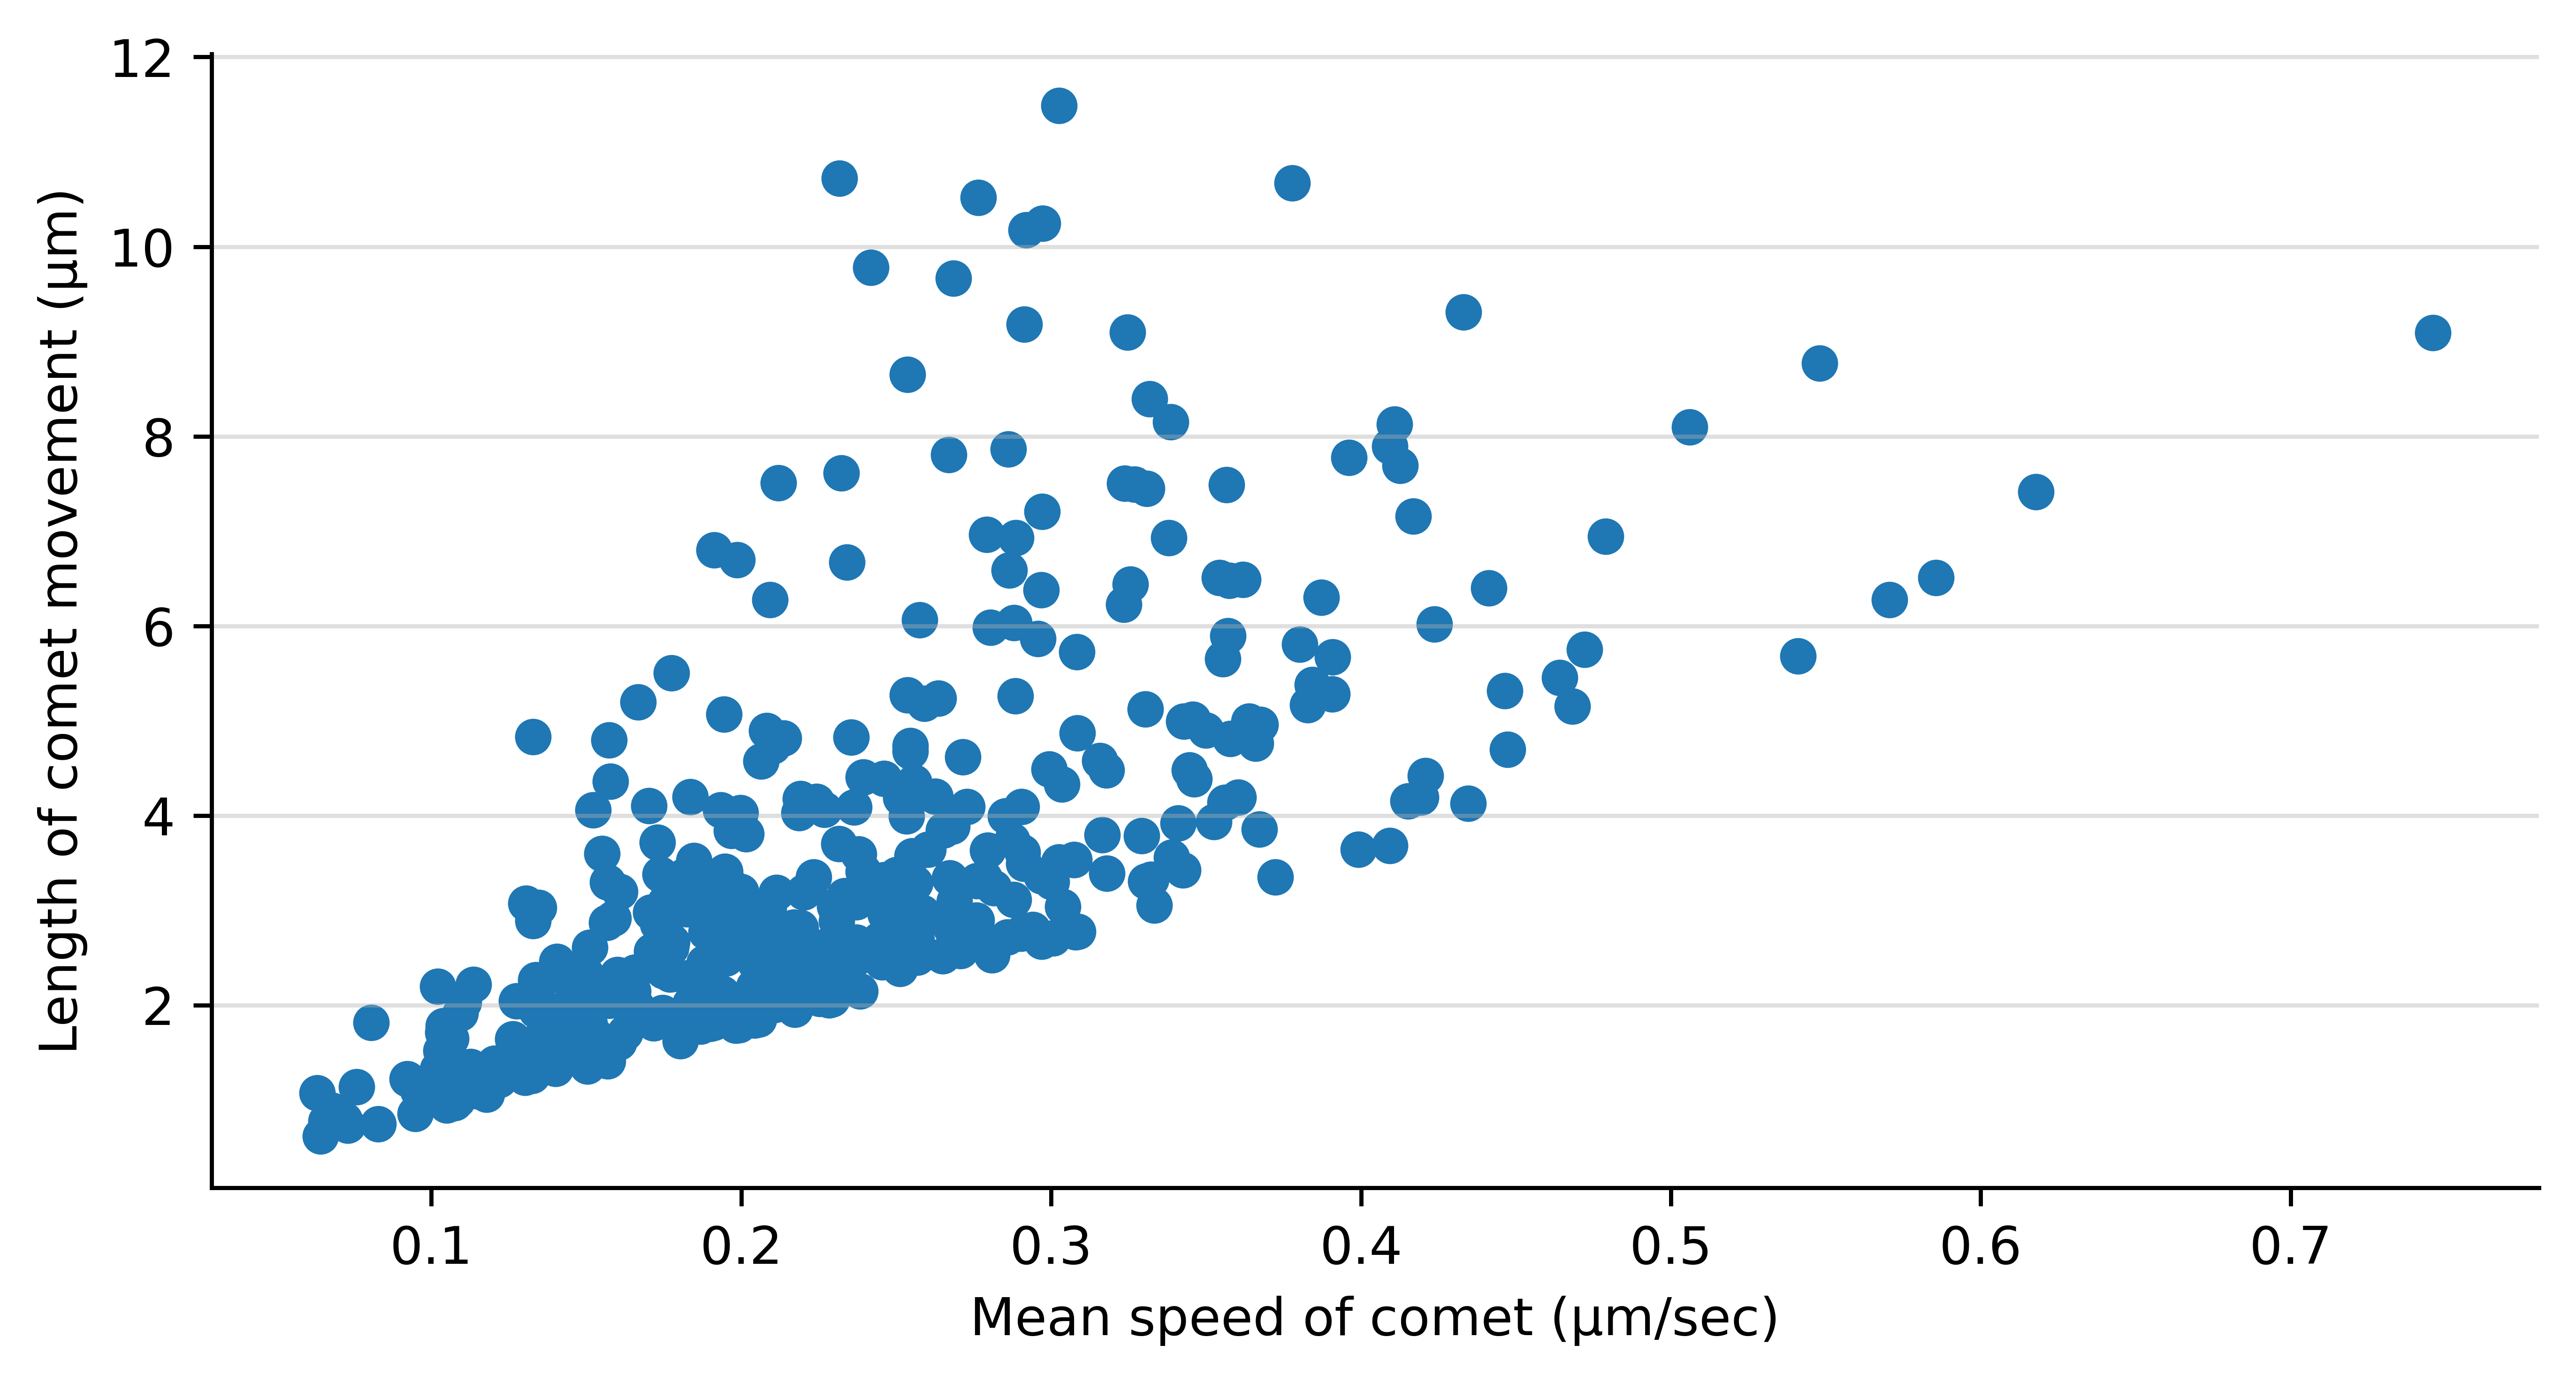
\includegraphics[width=\textwidth]{analysis/reports/distance_vs_meanspeed.png}
			\caption{COS-7 cells MT comets; correlation between length of EB3-GFP comet movement and it's mean speed} 
			\label{mt_live} 
		\end{minipage}
	\end{center}
\end{figure}

To get a better insight into the distributions of these values, we created a violin-plot, which visualizes the statistical analysis of the data (Fig. \ref{prob_density})

% Estimated probability density 
\begin{figure}[h!]
	\begin{center}
		\begin{minipage}{0,8\textwidth}
			
			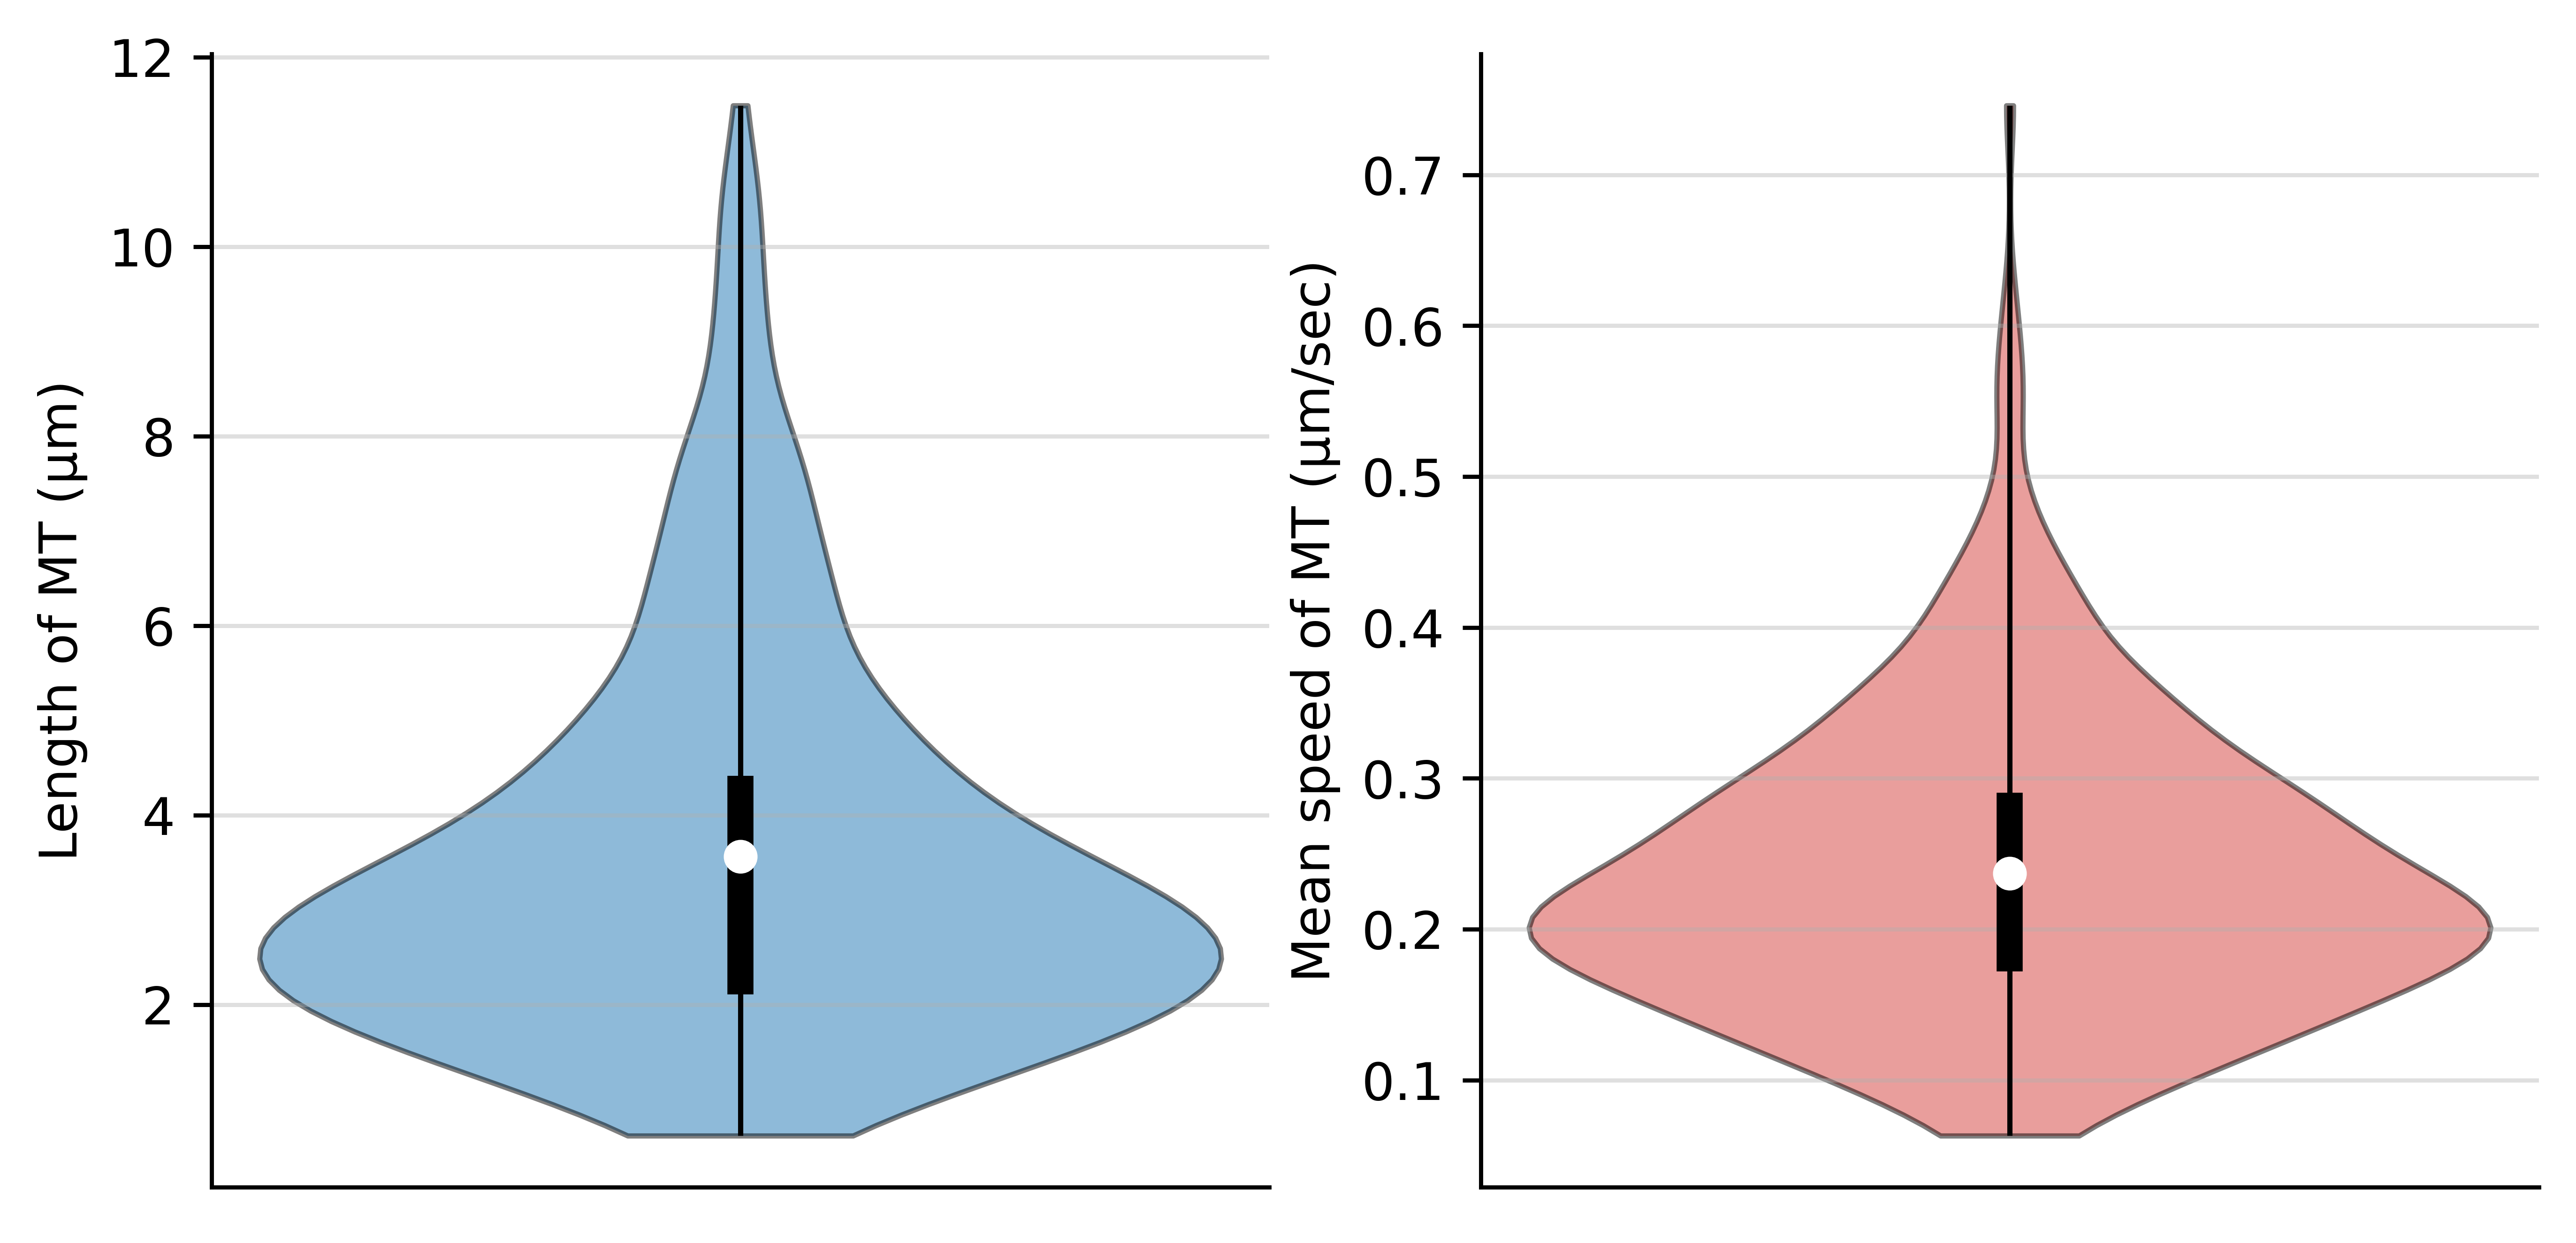
\includegraphics[width=\textwidth]{analysis/reports/prob_density.png}
			\caption{\textbf{probability density estimation} for finding a EB3 comet with a specific value; white dot: mean value; thick black line: area over the first and third quartile; whiskers: range of the measured values} 
			\label{prob_density} 
		\end{minipage}
	\end{center}
\end{figure}
\\
Based on Fig. \ref{mt_live} we furthermore calculated the overall mean speed and mean total travel length of the comets inside the COS-7 cell Tab. \ref{tab:comet}

\begin{table}[h] 
    \footnotesize
    \begin{center}
        \caption{statistical properties of the EB3 comet movements}
        \begin{tabular} {c c c l l l l l}
            & mean length [$\mu m$]&  mean speed [$\mu m s^{-1}$] \\ \hline
            COS-7 cell & 3.564 & 0.237  \\ \hline 
        \end{tabular}
        \label{tab:comet}
    \end{center}
\end{table}



\subsection{MT acetylation immunocytochemistry}
Alexa Fluor 568 is the fluorophore of the acetylated MT and Atto647N tagged the total $\alpha$-tubulin in the C-terminal end. We sampled both color channels with an exposure time of 300ms in a wide-field imaging process. Additionally, to get more structural information about the cells, DAPI and GFP were measured with an exposure time of 100ms. (Fig. \ref{whole_cell})

\begin{figure}[h!]
	\begin{center}
		\begin{minipage}{0,8\textwidth}
			
			\includegraphics[width=\textwidth]{analysis/reports/overlay_cell1.png}
			\caption{COS-7 cells; red (exposure time of 300ms): acetylated tubulin; yellow (exposure time of 300ms; self-labed antibody Anti‐tubulin‐Atto647N): total tubulin; green (exposure time of 100ms) : actin filament; blue (exposure time of 100ms): cell core} 
			\label{whole_cell} 
		\end{minipage}
	\end{center}
\end{figure}

With the help of the structural informations of DAPI and GFP, each cell was analysed by it's mCherry and Atto647N fluorescence intensity with the software Fiji by measuring the corresponding tubulin area. From this collected data we calculated the ratio between the acetylated and the total tubulin (Fig. \ref{acetylated_tubulin})

\begin{figure}[h!]
	\begin{center}
		\begin{minipage}{0,8\textwidth}
			
			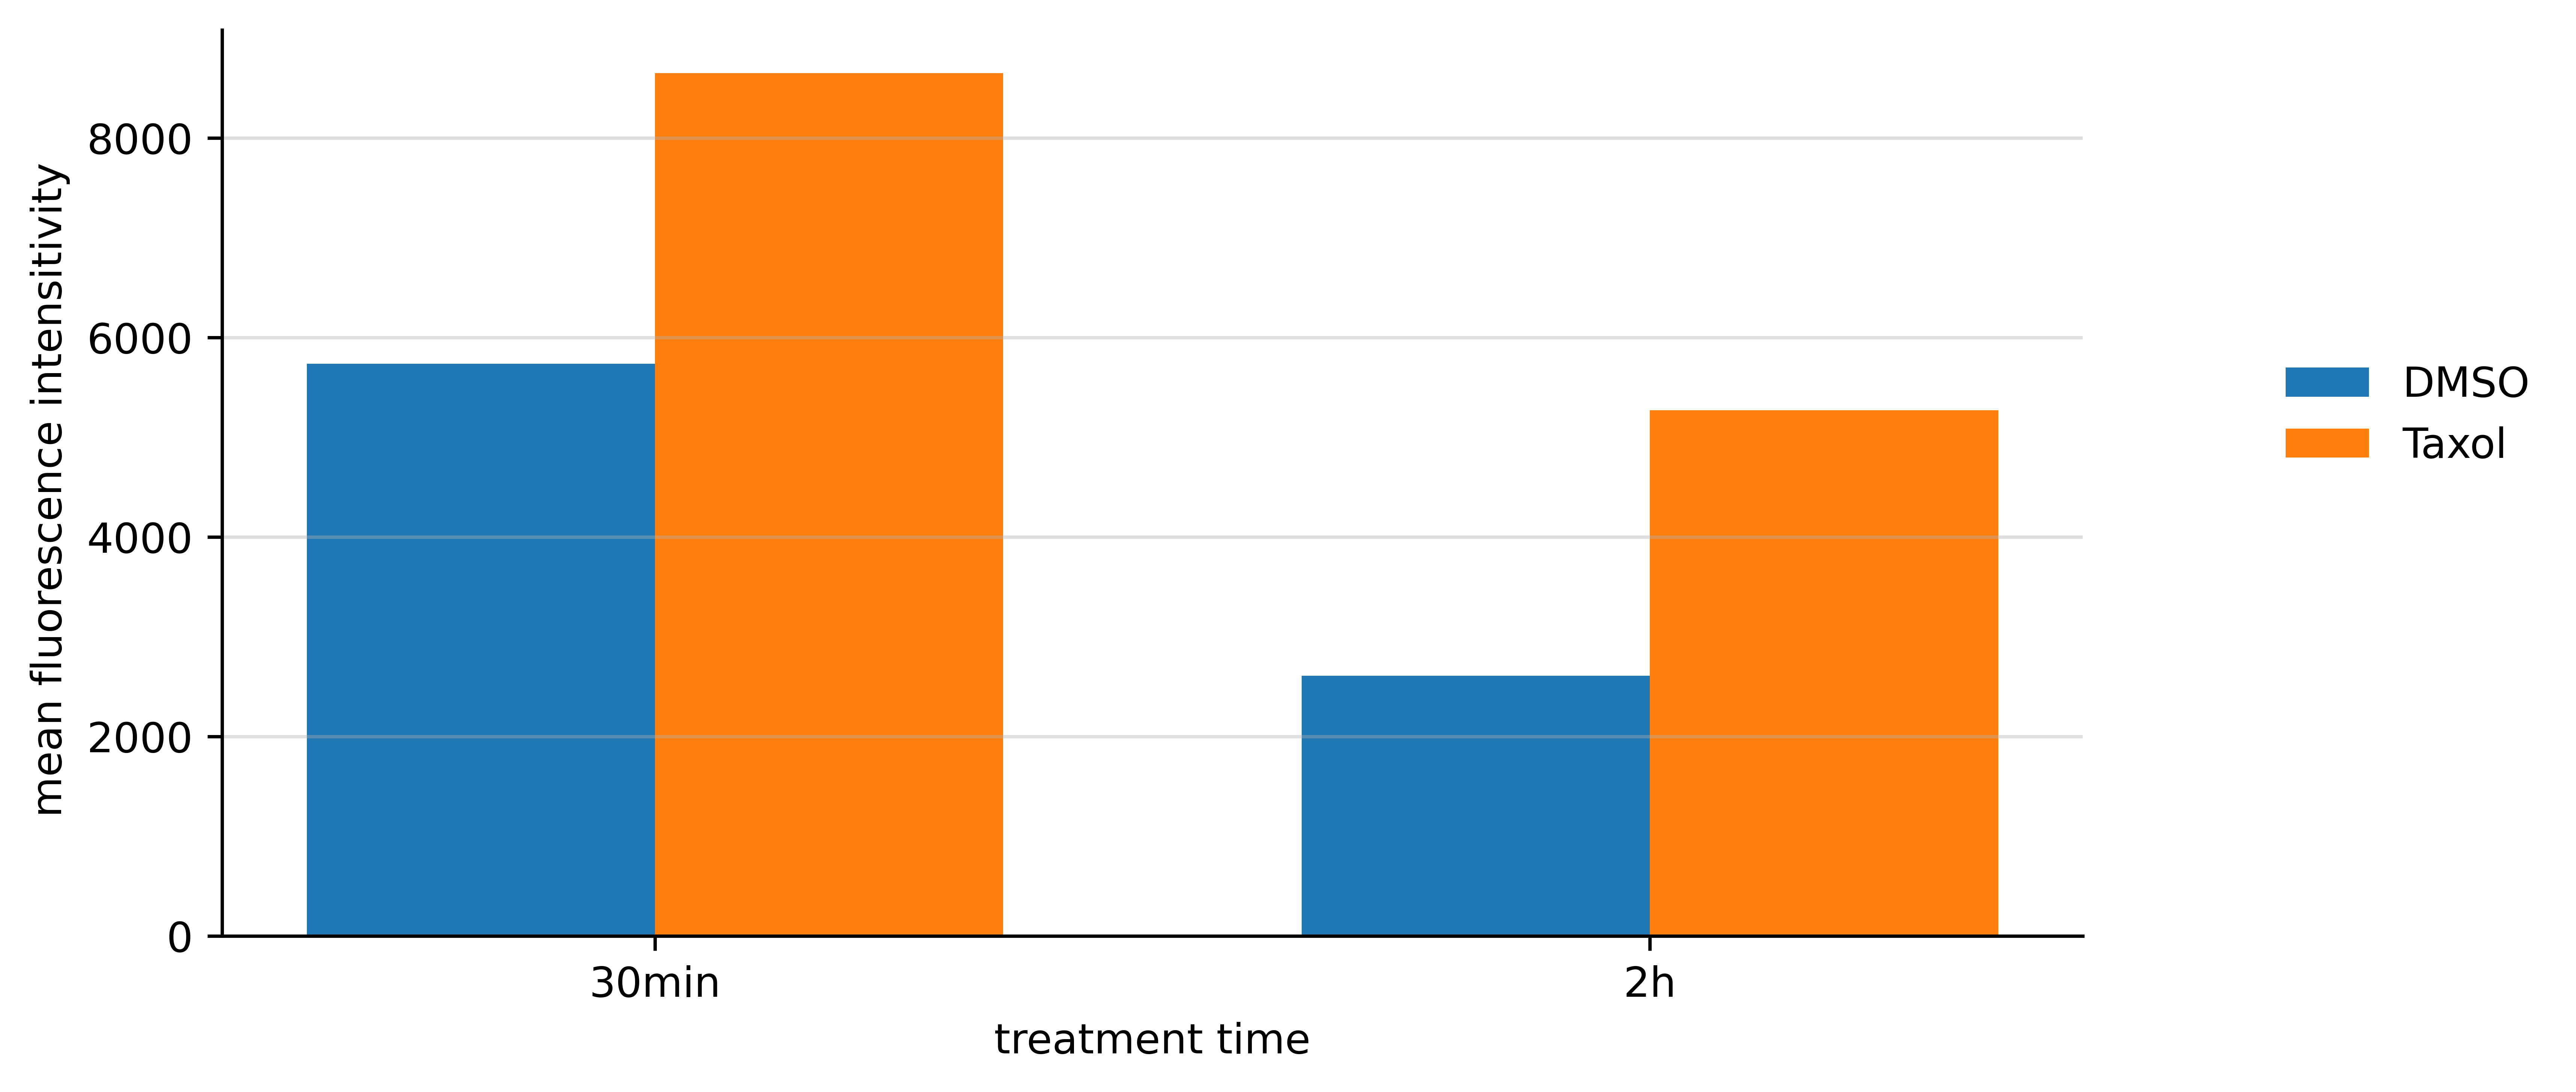
\includegraphics[width=\textwidth]{analysis/reports/acetylated_tubulin.png}
			\caption{ratio of acetylated tubulin to total tubulin} 
			\label{acetylated_tubulin} 
		\end{minipage}
	\end{center}
\end{figure}

